\documentclass{article}
\usepackage[utf8]{inputenc}
\usepackage{physics}
\usepackage{amsmath}
\usepackage{showlabels}
\title{Statistical Computing for Scientists and Engineers\\[1em] Homework 2}
\author{Jiale Shi}
\date{September/21/2018}

\usepackage{natbib}
\usepackage{graphicx}
\usepackage{array}
\begin{document}
\maketitle

\newpage
\section{Problem 1}
(a) Obtain analytic forms of:
The posterior distribution of Eq. (3) and the marginal posterior distribution over $\alpha$ and $\beta$:$p(\alpha,\beta|y)$ by using Eq. (4), Eq.(5) and the hint provided.

Answer:
\begin{equation}
\begin{aligned}
    p(\theta,\alpha,\beta|y) & \propto p(\alpha,\beta) p(\theta|\alpha,\beta)p(y|\theta,\alpha,\beta) \\
    & \propto (\alpha+\beta)^{-5/2}\prod_{j=1}^{J} \frac{\Gamma(\alpha+\beta)}{\Gamma(\alpha)\Gamma(\beta)}\theta_{j}^{\alpha+y_{j}-1}(a-\theta_{j})^{\beta+n_{j}-y_{j}-1}
\end{aligned}
\end{equation}

\begin{equation}
\begin{aligned}
    p(\alpha,\beta|y) & = \frac{ p(\theta,\alpha,\beta|y)}{ p(\theta|\alpha,\beta,y)} \\
    & \propto \frac{(\alpha+\beta)^{-5/2}\prod_{j=1}^{J} \frac{\Gamma(\alpha+\beta)}{\Gamma(\alpha)\Gamma(\beta)}\theta_{j}^{\alpha+y_{j}-1}(a-\theta_{j})^{\beta+n_{j}-y_{j}-1}}{ \prod_{j=1}^{J} \frac{\Gamma(\alpha+\beta+n_{j})}{\Gamma(\alpha+y_{j})\Gamma(\beta+n_{j}-y_{j})}\theta_{j}^{\alpha+y_{j}-1}(a-\theta_{j})^{\beta+n_{j}-y_{j}-1} } \\
     & \propto \frac{(\alpha+\beta)^{-5/2}\prod_{j=1}^{J} \frac{\Gamma(\alpha+\beta)}{\Gamma(\alpha)\Gamma(\beta)}}{ \prod_{j=1}^{J} \frac{\Gamma(\alpha+\beta+n_{j})}{\Gamma(\alpha+y_{j})\Gamma(\beta+n_{j}-y_{j})}} \\
\end{aligned}
\end{equation}

(b) Plot the marginal posterior density $p(\alpha,\beta|y)$ as a function of the transformed variables $\log(\frac{\alpha}{\beta})$ and $\log(\alpha+\beta) \in [(-1.3,-2.3);(1,5)]$. Obtain the corresponding value of $(\alpha,\beta)$.

Answer:
Let $X = \log{\frac{\alpha}{\beta}}, Y = \log(\alpha+\beta)$. Then $\beta = \frac{\exp(Y)}{1+\exp(X)}, \alpha = \exp(X)\beta$.
Using the python code that provided to us. 
\begin{figure}[ht]
\centering
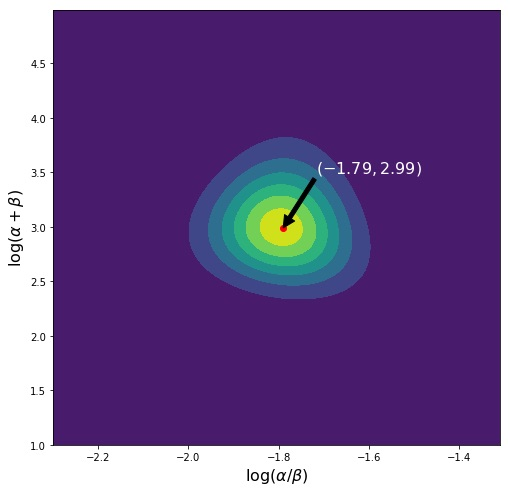
\includegraphics[scale=0.5]{hw2_1b.jpg}
\caption{the marginal posterior density $p(\alpha,\beta|y)$ as a function of the transformed variables $\log(\frac{\alpha}{\beta})$ and $\log(\alpha+\beta)$}
%\label{fig:universe}
\end{figure}

$X = -1.79, Y = 2.99$,then the corresponding value of $(\alpha,\beta) = (2.85,17.04)$


\newpage
\section{Problem 2}
Jeffrey's prior and maximum entropy prior: Consider a random variable $x$ described by a Possion distribution:

\begin{equation}
    x \sim p(x;\theta) = \frac{\theta^x e^{-\theta}}{x!}
\end{equation}
(a) Determine the Jeffrey prior $\pi^{J}$ for $\theta$. Is the scale invariant prior $\pi_{0}(\theta) = \frac{1}{\theta}$ preferable to $\pi^{J}$? Why?


Answer:
\begin{equation}
   p(x|\theta) = \frac{\theta^x e^{-\theta}}{x!}
\end{equation}
Therefore,
\begin{equation}
   I(\theta) = -E\left[\frac{\partial^2}{\partial \theta^2} \ln p(x|\theta)\right] = \frac{\theta}{\theta^2} = \frac{1}{\theta}
\end{equation}

Therefore the Jeffreys' prior is given by:
\begin{equation}
   \pi^J = \left[I(\theta)\right]^{1/2} = \theta^{-1/2}
\end{equation}

The scale invariant prior $\pi_{0}(\theta) = \frac{1}{\theta}$ is not preferable to $\pi^{J}$ because they are not the same function.

(b) Find the maximum entropy prior for $\theta$ for the reference measure $\pi^J$ subject to the constraints $E^{\pi}[\theta] = 1$, $Var^{\pi}[\theta] = 1$. 

Answer: considering the reference measure as $\pi_{ref}=\pi^J \propto \theta^{-1/2}$.

The maximum entropy prior under the constraints that the prior mean and variance of $\theta$ are both 1:

Two constrains, therefore,$K=2$.

$E^{\pi}[\theta] = 1$, $g_{1}(\theta)=\theta$.

$Var^{\pi}[\theta] = 1= E[(\theta-1)^2]$, $g_{2}(\theta)=(\theta-1)^2$.

\begin{equation}
\hat{\pi} = \frac{\pi_{ref}(\theta)\exp(\sum_{k=1}^{K} \lambda_{k}g_{k}(\theta))}{\int \pi_{ref}(\theta)\exp(\sum_{k=1}^{K} \lambda_{k}g_{k}(\theta))}
\end{equation}

In this problem,
\begin{equation}
\hat{\pi} \propto \theta^{-1/2} \exp(\lambda_{1}\theta+\lambda_{2}(\theta-1)^2)  
\end{equation}

(c) Find the maximum entropy prior for $\theta$ for the reference measure $\pi_0$ subject to the constraints $E^{\pi}[\theta] = 1$, $Var^{\pi}[\theta] = 1$. 

Answer: Considering the reference measure as $\pi_{ref}=\pi_{0} \propto \theta^{-1}$.

The maximum entropy prior under the constraints that the prior mean and variance of $\theta$ are both 1:

Two constrains, therefore,$K=2$.

$E^{\pi}[\theta] = 1$, $g_{1}(\theta)=\theta$.

$Var^{\pi}[\theta] = 1= E[(\theta-1)^2]$, $g_{2}(\theta)=(\theta-1)^2$.

\begin{equation}
\hat{\pi} = \frac{\pi_{ref}(\theta)\exp(\sum_{k=1}^{K} \lambda_{k}g_{k}(\theta))}{\int \pi_{ref}(\theta)\exp(\sum_{k=1}^{K} \lambda_{k}g_{k}(\theta))}    
\end{equation}

In this problem,
\begin{equation}
\hat{\pi} \propto \theta^{-1} \exp(\lambda_{1}\theta+\lambda_{2}(\theta-1)^2)  
\end{equation}

\newpage
\section{Problem 3}
Laplace approximation: the data set $X= (X_1,...,X_n)$ presents the number of the wins of a football team in the past n home games. We can model this using 
\begin{equation}
    X_{i} \sim g(x_{i}|\theta) = \theta (\theta+1)x_{i}^{\theta -1}(1-x_{i}), x_{i} = (0,1)
\end{equation}
with parameter $\theta > 0$. Unfortunately, this model does not have any corresponding, useful, conjugate prior. But it is acceptable to impose a prior model on $\theta$ with Gamma distribution.

(a) Derive the posterior PDF of $\theta$.

Answer:
\begin{equation}
\begin{aligned}
    p(\theta | x) &= Gamma(\theta;a,b) \prod_{i=1}^{n}p(x_{i}|\theta) \\
    &= \frac{b^{a}\theta^{a-1}\exp{-b\theta}}{\Gamma(a)}\theta^{n}(\theta+1)^{n}\prod_{i=1}^{n}x_{i}^{\theta-1}(1-x_{i})
\end{aligned}
\end{equation}

(b) Using Laplace approximation, find a normal distribution but approximates the posterior distribution using n = 20.
\begin{equation}
    \sum_{x=i} \ln X_{i} = -4.59
\end{equation}
and a = b = 1 where a and b are the hyperparameters of the gamma distribution $Gamma(a,b)$.

Answer:

\begin{math}
n = 20; a=b=1
\end{math}

\begin{equation}
\begin{aligned}
    p(\theta | x) 
    &= \frac{\exp{-\theta}}{\Gamma(1)}\theta^{20}(\theta+1)^{20}\prod_{i=1}^{20}x_{i}^{\theta-1}(1-x_{i})
\end{aligned}
\end{equation}

\begin{equation}
\begin{aligned}
    \log p(\theta | x) 
    &= -\theta + 20 \log(\theta(\theta+1))+(\theta-1)\sum_{i}^{20}\log(x_{i})+C
\end{aligned}
\end{equation}

the first derivative
\begin{equation}
\begin{aligned}
    \frac{d \log p(\theta | x) }{d \theta}
    &= -1 + \frac{20}{\theta} +\frac{20}{\theta+1}+\sum_{i}^{20}\log(x_{i}) = 0
\end{aligned}
\end{equation}

\begin{equation}
\begin{aligned}
    \theta^{MAP} \approx 6.69
\end{aligned}
\end{equation}

the second derivative
\begin{equation}
\begin{aligned}
    A = -\frac{d^2 \log p(\theta | x) }{d \theta^2}{\theta=\theta^{MAP}=6.69}
    &= - \frac{20}{\theta^2} -\frac{20}{(\theta+1)^2} \approx -(-0.785) = 0.785 = \frac{1}{\sigma^2}
\end{aligned}
\end{equation}

Therefore,

\begin{equation}
\begin{aligned}
    p(\theta | x) 
    &\approx (2\pi)^{-10} |A|^{1/2}\exp{-\frac{1}{2}(\theta - \theta^{MAP})^{2} A} \\
    &\approx (2\pi)^{-10} (0.785)^{1/2}\exp{-\frac{1}{2}(\theta - 6.69)^{2} 0.785} \\
    &\approx (2\pi)^{-10} (\frac{1}{\sigma^2})^{1/2}\exp{-\frac{1}{2\sigma^2}(\theta - \theta^{MAP})^{2} }
\end{aligned}
\end{equation}

where $\frac{1}{\sigma^2}= 0.785,\theta^{MAP}=6.69 $

\newpage
\section{Problem 4}
Monte Carlo integration: Consider the following function,
\begin{equation}
    f(x) = x^{3} + 5x \cos{x}
\end{equation}

(a) Calculate the integral $I = \int_{a}^{b} f(x) d x$ with $a = 3$ and $b = 4$ using Monte Carlo integration with $N = 10000$ samples. Compare this value with the exact solution.

Answer:
\begin{equation}
\begin{aligned}
I_{exact} &= \int_{a}^{b} f(x) d x \\
&= \int_{a}^{b} (x^{3} + 5x \cos{x}) d x \\
&=  \left[\frac{x^{4}}{4} +5x\sin{x}+5\cos{x}\right]\mid_{a}^{b}  \\
& = \left[\frac{x^{4}}{4} +5x\sin{x}+5\cos{x}\right]\mid_{3}^{4}\\
& \approx 28.178894351627594
\end{aligned}
\end{equation}

Using Monte Carlo integration with $N=10,000$ samples.
using the python's function numpy.random.uniform(3,4,10000).

The integral $I$ from Monte Carlo integration
\begin{equation}
I_{MC} = 28.192521342751455 \approx  I_{exact}
\end{equation}
the error is about 0.05$\%$.

\begin{figure}[ht]
\centering
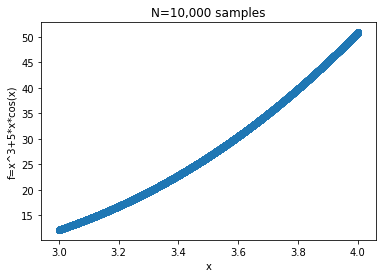
\includegraphics[scale=0.6]{HW2_P4_a.png}
\caption{Monte Carlo integration for P4a with N= 10,000}
%\label{fig:universe}
\end{figure}

(b) Check the relation between the number of samples $N$ and solution accuracy by plotting the error for $N = [10,1000]$.

Answer:

%See Figure 3
\begin{figure}[ht]
\centering
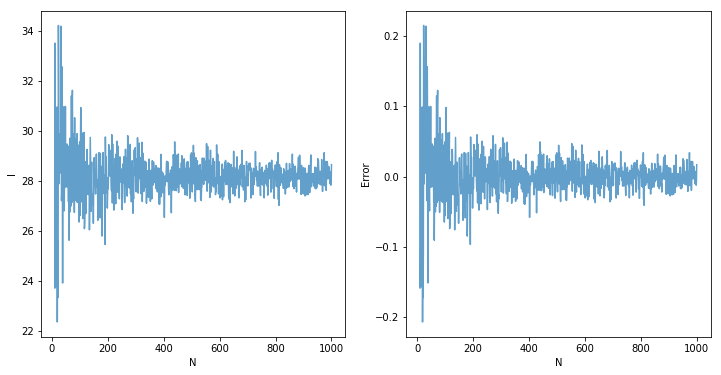
\includegraphics[scale=0.5]{HW2_P4_b.png}
\caption{a. Integral I for N = [10,1000]
b. Error for N = [10,1000]}
%\label{fig:universe}
\end{figure}

From the plot, we find that when N is small, the error is very large, but when N increases, the error becomes smaller.

\newpage
(c) For $N = 100, 1000, 10000$ and $100000$ repeat the MC integration for  m = 10000 times. Plot the histogram of the results of MC integration for each $N$. Use the law of large numbers to justify the trend in the histograms.

Answer:

\begin{figure}[ht]
\centering
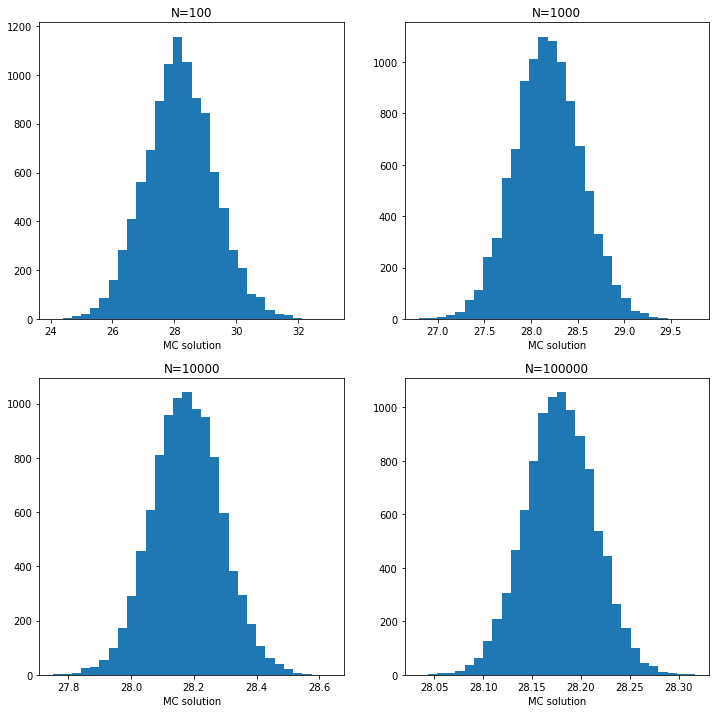
\includegraphics[scale=0.5]{HW2_P4_c.png}
\caption{Histogram of the results of MC for each N}
%\label{fig:universe}
\end{figure}

Using the law of large numbers to justify the trend in the histogram.
$Var[\Bar{X_{N}}] = \frac{\sigma^2}{N}$, therefore when N increases, $Var[\Bar{X_{N}}]=\frac{\sigma^2}{N}$ decreases, the histogram becomes more like a Gaussian distribution.

\newpage
\section{Problem 5}
Bayesian Information Criterion (BIC): suppose we toss a biased coin where probability of heads ($x=1$) is $\theta_{1}$. However, we only know about the outcome through an unreliable friend of ours, Joey, who can be trusted with a probability $\theta_{2}$. Let us call this report $y$. This means that we can write down $p(y|x,\theta_{2})$ as

(a) What is the joint probability distribution $p(x,y|\theta_{1},\theta_{2}$? Write your name in a table.

Answer:

\begin{center}
\begin{tabular}{ c c c }
   & y=0 & y=1 \\ 
x=0 & $(1-\theta_{1})\theta_{2}$ & $(1-\theta_{1})(1-\theta_{2})$ \\  
x=1 & $\theta_{1}(1-\theta_{2})$ & $\theta_{1}\theta_{2}$  
\end{tabular}
\end{center}

(b) Consider we have the outcomes
\begin{equation}
\begin{aligned}
    x = (1,1,0,1,1,0,0) \\
    x = (1,0,0,0,1,0,1)
\end{aligned}
\end{equation}

Find the maximum likelihood estimate for $\theta_{1}$ and $\theta_{2}$.

\begin{equation}
    p(\theta_{1},\theta_{2}|X,Y) = \theta_{1}^{4}(1-\theta_{1})^{3}\theta_{2}^{4}(1-\theta_{2})^{3}
\end{equation}

\begin{equation}
    \log p(\theta_{1},\theta_{2}|X,Y) = 4\log{\theta_{1}}+3\log{(1-\theta_{1})}+4\log{\theta_{2}}+3\log{(1-\theta_{2})}
\end{equation}

\begin{equation}
    \frac{\log p}{d \theta_{2}} = \frac{4}{\theta_{2}}-\frac{3}{1-\theta_{2}} = 0; \theta_{2}= \frac{4}{7}
\end{equation}

\begin{equation}
    \frac{\log p}{d \theta_{1}} = \frac{4}{\theta_{1}}-\frac{3}{1-\theta_{1}} = 0; \theta_{1}= \frac{4}{7}
\end{equation}

(c)We denote this model with $M_2$, where index 2 stands for the number of parameters in the model. Find $p(D|\hat{\theta_{1}},\hat{\theta_{2}},M_2)$ where $\hat{\theta}$ denotes the MLE solution for parameter $\theta$.

Answer:

From b, $\theta_{1}= \frac{4}{7}$ and $\theta_{2}= \frac{4}{7}$
\begin{center}
\begin{tabular}{ c c c }
   & y=0 & y=1 \\ 
x=0 & $\frac{12}{49}$ & $\frac{9}{49}$ \\  
x=1 & $\frac{12}{49}$ & $\frac{16}{49}$  
\end{tabular}
\end{center}

\begin{equation}
    p(X,Y|\theta_{1},\theta_{2},M_{2})= (\frac{4}{7})^{8}(\frac{3}{7})^{6} \approx 7.044 \times 10^{-5}
\end{equation}

(d) If we also denote a model with 4 parameters $\Bar{\theta} = (\theta_{0,0},\theta_{0,1},\theta_{1,0},\theta_{1,1})$ that represents $p(x,y|\Bar{\theta}) = \theta_{x,y}$. Find the MLE of $\Bar{\theta}$.

Answer:

\begin{center}
\begin{tabular}{ c c c }
   & y=0 & y=1 \\ 
x=0 & $\theta_{0,0}$ & $\theta_{0,1}$ \\  
x=1 & $\theta_{1,0}$ & $\theta_{1,1}$  
\end{tabular}
\end{center}

\begin{equation}
\begin{aligned}
    &p(\Bar{\theta}|X,Y) = \theta_{0,0}^{2} \theta_{0,1} \theta_{1,0}^{2} \theta_{1,1}^{2}\\ 
    &\theta_{0,1} = 1- \theta_{0,0}-\theta_{1,0}-\theta_{1,1}
\end{aligned}
\end{equation}

\begin{equation}
\begin{aligned}
    p(\Bar{\theta}|X,Y) = \theta_{0,0}^{2} (1- \theta_{0,0}-\theta_{1,0}-\theta_{1,1}) \theta_{1,0}^{2} \theta_{1,1}^{2}
\end{aligned}
\end{equation}

\begin{equation}
\begin{aligned}
    \log p = 2\log\theta_{0,0} +\log(1- \theta_{0,0}-\theta_{1,0}-\theta_{1,1}) +2\log \theta_{1,0} +2\log \theta_{1,1}
\end{aligned}
\end{equation}

\begin{equation}
\begin{aligned}
    \frac{d \log p}{d \theta_{0,0}} = \frac{2}{\theta_{0,0}} - \frac{1}{1- \theta_{0,0}-\theta_{1,0}-\theta_{1,1}}=0
\end{aligned}
\end{equation}

\begin{equation}
\begin{aligned}
    \frac{d \log p}{d \theta_{1,0}} = \frac{2}{\theta_{1,0}} - \frac{1}{1- \theta_{0,0}-\theta_{1,0}-\theta_{1,1}}=0
\end{aligned}
\end{equation}

\begin{equation}
\begin{aligned}
    \frac{d \log p}{d \theta_{1,1}} = \frac{2}{\theta_{1,1}} - \frac{1}{1- \theta_{0,0}-\theta_{1,0}-\theta_{1,1}}=0
\end{aligned}
\end{equation}

\begin{equation}
\begin{aligned}
    & \theta_{0,0}=\frac{2}{7} \\
    & \theta_{0,1}=\frac{1}{7} \\
    & \theta_{1,0}=\frac{2}{7} \\
    & \theta_{1,1}=\frac{2}{7} 
\end{aligned}
\end{equation}
(e) Find $p = (D|\hat{\theta}, M_4)$ where $\hat{\theta}$ denotes the MLE solution for parameters $\Bar{\theta}$.

Answer:

\begin{center}
\begin{tabular}{ c c c }
   & y=0 & y=1 \\ 
x=0 & $\frac{2}{7}$ & $\frac{1}{7}$ \\  
x=1 & $\frac{2}{7}$ & $\frac{2}{7}$  
\end{tabular}
\end{center}

\begin{equation}
    p(X,Y|\theta_{0,0},\theta_{0,1},\theta_{1,0},\theta_{1,1},M_{2})= (\frac{2}{7})^{6}(\frac{1}{7}) \approx 7.771 \times 10^{-5}
\end{equation}

(f) Find the Bayesian Information Criterion for $M_2$ and $M_4$. Which model is preferred by this criterion?

Answer:
From the Bayesian Information Criterion for $M_2$ and $M_4$,

For $M_2$,$k=2, N=7, L = p(X,Y|\theta_{1},\theta_{2},M_{2})= (\frac{4}{7})^{8}(\frac{3}{7})^{6} \approx 7.044 \times 10^{-5} $
\begin{equation}
    BIC =  k\log(N) -2 \log (L) \approx 23.01 
\end{equation}

For $M_4$,$k=3$(there is a constrain for the four parameters, therefore only three parameters are free parameters, and k should be 3), $N=7$, $L =  p(X,Y|\theta_{0,0},\theta_{0,1},\theta_{1,0},\theta_{1,1},M_{2})= (\frac{2}{7})^{6}(\frac{1}{7}) \approx 7.771 \times 10^{-5} $
\begin{equation}
    BIC =  k\log(N) -2 \log (L) \approx 24.76
\end{equation}

Since $BIC_{M_4} > BIC_{M_2} $, $M_2$ is more preferred by this criterion.

\newpage
\section{Problem 6}
Maximum Likelihood Estimation (MLE) and Maximum A Posterior (MAP):
Consider a random variable $x$ described by 

(a) Derive the maximum likelihood estimate (MLE) ($\lambda_{MLE}$)

Answer:
The likelihood is given by
\begin{equation}
p(x|\lambda) = \prod_{i=1}^{n} \lambda \exp{-\lambda x_{i}}
\end{equation}
The log likelihood:
\begin{equation}
    \ln{p} = n \ln{\lambda} -\lambda \sum{x_i}
\end{equation}
Now set set derivative w.r.t $\lambda$ to $0$:
\begin{equation}
    \frac{d \ln{p}}{d \lambda} = \frac{n}{\lambda} + \sum{x_i} =0
\end{equation}
Therefore,
\begin{equation}
    \lambda_{MLE} = \frac{1}{\Bar{x}}. \left( \Bar{x} = \frac{1}{n} \sum_{i=1}^{n} x_{i} \right)
\end{equation}

(b)Obtain an analytic form of the posterior distribution of Eq.(11) and Derive the maximum a posterior estimator (MAP) $\lambda_{MAP}$ as a function of $\alpha,\beta$.

Answer:
Let us consider the data $X = x_{1},x_{2},...,x_{n}$. The posterior distribution $p(\lambda | X)$ is given by:
\begin{equation}
\begin{aligned}
p(\lambda | X) &= \frac{p(\lambda | X) p(\lambda)}{\int p(\lambda | X) p(\lambda)} \\
& \propto p(\lambda | X) p(\lambda) \\
& \lambda^{n} \exp{-\lambda \sum_{i=1}^{N} x_{i}} Gamma(\alpha,\beta) \\
& \lambda^{n} \exp{-\lambda \sum_{i=1}^{N} x_{i}} \lambda^{\alpha-1}\exp{-\beta \lambda} \\
& e^{-\lambda(\sum_{i=1}^{N} x_{i}+\beta)} \lambda^{n+\alpha-1}
\end{aligned}
\end{equation}

\begin{equation}
p(\lambda | X) \propto Gamma(\alpha+n,\sum_{i=1}^{N} x_{i}+\beta )  
\end{equation}

The log posterior:
\begin{equation}
\log p(\lambda | X) \propto -\lambda(\sum_{i=1}^{N} x_{i}+\beta)+(n+\alpha-1)\log \lambda
\end{equation}

\begin{equation}
0 = \frac{d \log p(\lambda | X) }{d \lambda} = -(\sum_{i=1}^{N} x_{i}+\beta)+ \frac{n+\alpha-1}{\lambda}
\end{equation}

\begin{equation}
\lambda_{MAP}= \frac{n+\alpha-1}{\sum_{i=1}^{N} x_{i}+\beta}
\end{equation}

(c) Generate $N=20$ samples drawn from an exponential distribution with parameter $\lambda = 0.2$. Fix $\beta = 100$ and vary $\alpha$ over the range(1,40) using a step-size of 1.

Compute the corresponding MLE and MAP estimates for $\lambda$

For each $\alpha$, compute the mean squared $error^2$ of both estimates compared against the true value and then plot the mean squared error as a function of $\alpha$.

Now, fix $\alpha= 30$, $\theta=100$ and vary N over the range(1,500) using a step-size of 1. Plot the mean squared error for each N of the corresponding estimates and explain under what condition is the MAP estimator better.

\begin{figure}[ht]
\centering
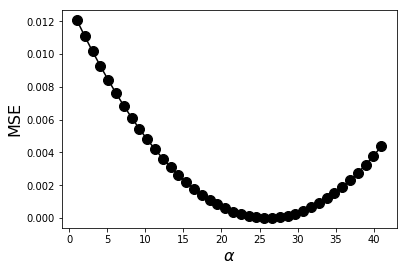
\includegraphics[scale=0.5]{HW2_P6_c1.png}
\caption{MSE as a function of $\alpha$}
%\label{fig:universe}
\end{figure}

\begin{figure}[ht]
\centering
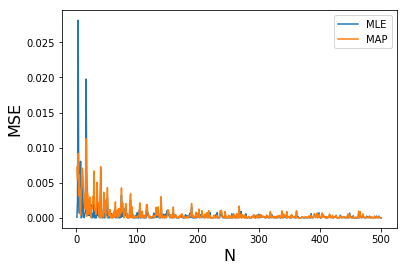
\includegraphics[scale=0.5]{HW2_P6_c2.png}
\caption{MSE as a function of N}
%\label{fig:universe}
\end{figure}

From Figure 6, when N is small, then the MAP estimator would be better than the MLE estimator.
%\bibliographystyle{plain}
%\bibliography{references}
\end{document}
